\documentclass[a4paper,12pt]{article}

% paquets pour avoir les lettres accentués et la typographie française
\usepackage{a4wide}
\usepackage[utf8]{inputenc}
\usepackage[frenchb]{babel}

%\usepackage{glossaries}



\usepackage[colorlinks=true,linkcolor=black]{hyperref}
\usepackage[T1]{fontenc}%la police utilisee dans le document

%trois package pour taper du texte mathémathiques
\usepackage{amsmath}
\usepackage{amssymb}
\usepackage{amsfonts}
\usepackage{mathrsfs}

%pour insérer des styles de liste supplémentaire
%\usepackage{enumerate}

%pour l'insertion d'image
\usepackage{graphicx}
\usepackage{float}% pour l'utilisation de "centering" et de l'option [H] qui permet de placer plus efficacement les images

%package pour les lien url :
\usepackage{url}


%pour l'insertion de code source


\usepackage{fancyvrb}

\begin{document}

%%%%%%%%%%%%%%%%%%%%%%%%%%%%%%%%%%%%%%%%%%%%%%%%%%%%
% PAGE DE GARDE
%%%%%%%%%%%%%%%%%%%%%%%%%%%%%%%%%%%%%%%%%%%%%%%%%%%%

\begin{titlepage}
\begin{flushleft}
\large{Universit\'e du Havre \\
Master Matis \\
Sp\'ecialisation SIRES\\
}
\end{flushleft}

\setlength{\parskip}{96pt}

\begin{center}
\huge\textbf{TeXloud\\Des documents \LaTeX ~dans le Cloud}

\setlength{\parskip}{18pt}
\large\textsc{Référent: Y. Pigné}

\setlength{\parskip}{70pt}

\Large\textbf{Rapport}

\setlength{\parskip}{50pt}

\large Adrien Bruyère\\David Ducatel\\Meva Rakotondratsima\\Sidina Biha\\Zakaria Bouchakor
\end{center}
\setlength{\parskip}{50pt}
\begin{flushleft}
\rule{.4mm}{26mm}\rule{105mm}{.4mm}
\today
\end{flushleft}
\end{titlepage}

%%%%%%%%%%%%%%%%%%%%%%%%%%%%%%%%%%%%%%%%%%%%%%%%%%%%
% FIN DE LA PAGE DE GARDE
%%%%%%%%%%%%%%%%%%%%%%%%%%%%%%%%%%%%%%%%%%%%%%%%%%%%
 
\clearpage

\tableofcontents

\newpage

\section{Introduction}
\subsection{Rappel du sujet}
\paragraph*{}
Ce projet propose la création et la gestion collaborative de documents
Latex. Le but est de proposer à des plateformes dépourvues de distribution
Latex (tablettes, smartphones, desktops), de se connecter au Web et
d'accéder à ces service de gestion et de compilation de documents.
\paragraph*{} 
Les utilisateurs seront authentifiés au service et bénéficieront d'un espace
de stockage privé. L'application facilitera le partage de documents et le
travail collaboratif entre utilisateurs du service.
\paragraph*{} 
Coté client, deux types d'applications seront développés :

\begin{itemize}
 \item Un service Web permettra l'accès au service à partir de n'importe
quelle machine (desktop, tablette non-Android) pourvue d'un navigateur
Web et d'une connexion internet

 \item Une application Android, permettra une certaine autonomie avec le
stockage temporaire d'une copie de travail des documents, permettant
un mode d'édition non-connecté.
\end{itemize}

\subsection{L'équipe}
\paragraph*{}
L'équipe est composé de 5 personnes:
\begin{itemize}
 \item Adrien Bruyère est responsable du développement de l'application Android
 \item David Ducatel (chef de projet) est responsable du développement de la frontale et du service de compilation.
 \item Meva Rakotondratsima est responsable du développement du service de stockage de données.
 \item Sidina Biha, Zakaria Bouchakor sont responsables du développement de l'application WEB
\end{itemize}

\newpage
\section{Choix techniques}
\subsection{Architecture général}
\paragraph*{}
Le projet est divisé en 5 parties minimum:
\begin{itemize}
 \item Un serveur web
 \item Une application Android
 \item Un serveur de routage et d'ordonnancement
 \item Un à N serveur(s) de stockage de données
 \item Un à N serveur(s) de compilation
\end{itemize}

\begin{figure}[!ht]
\begin{center}
  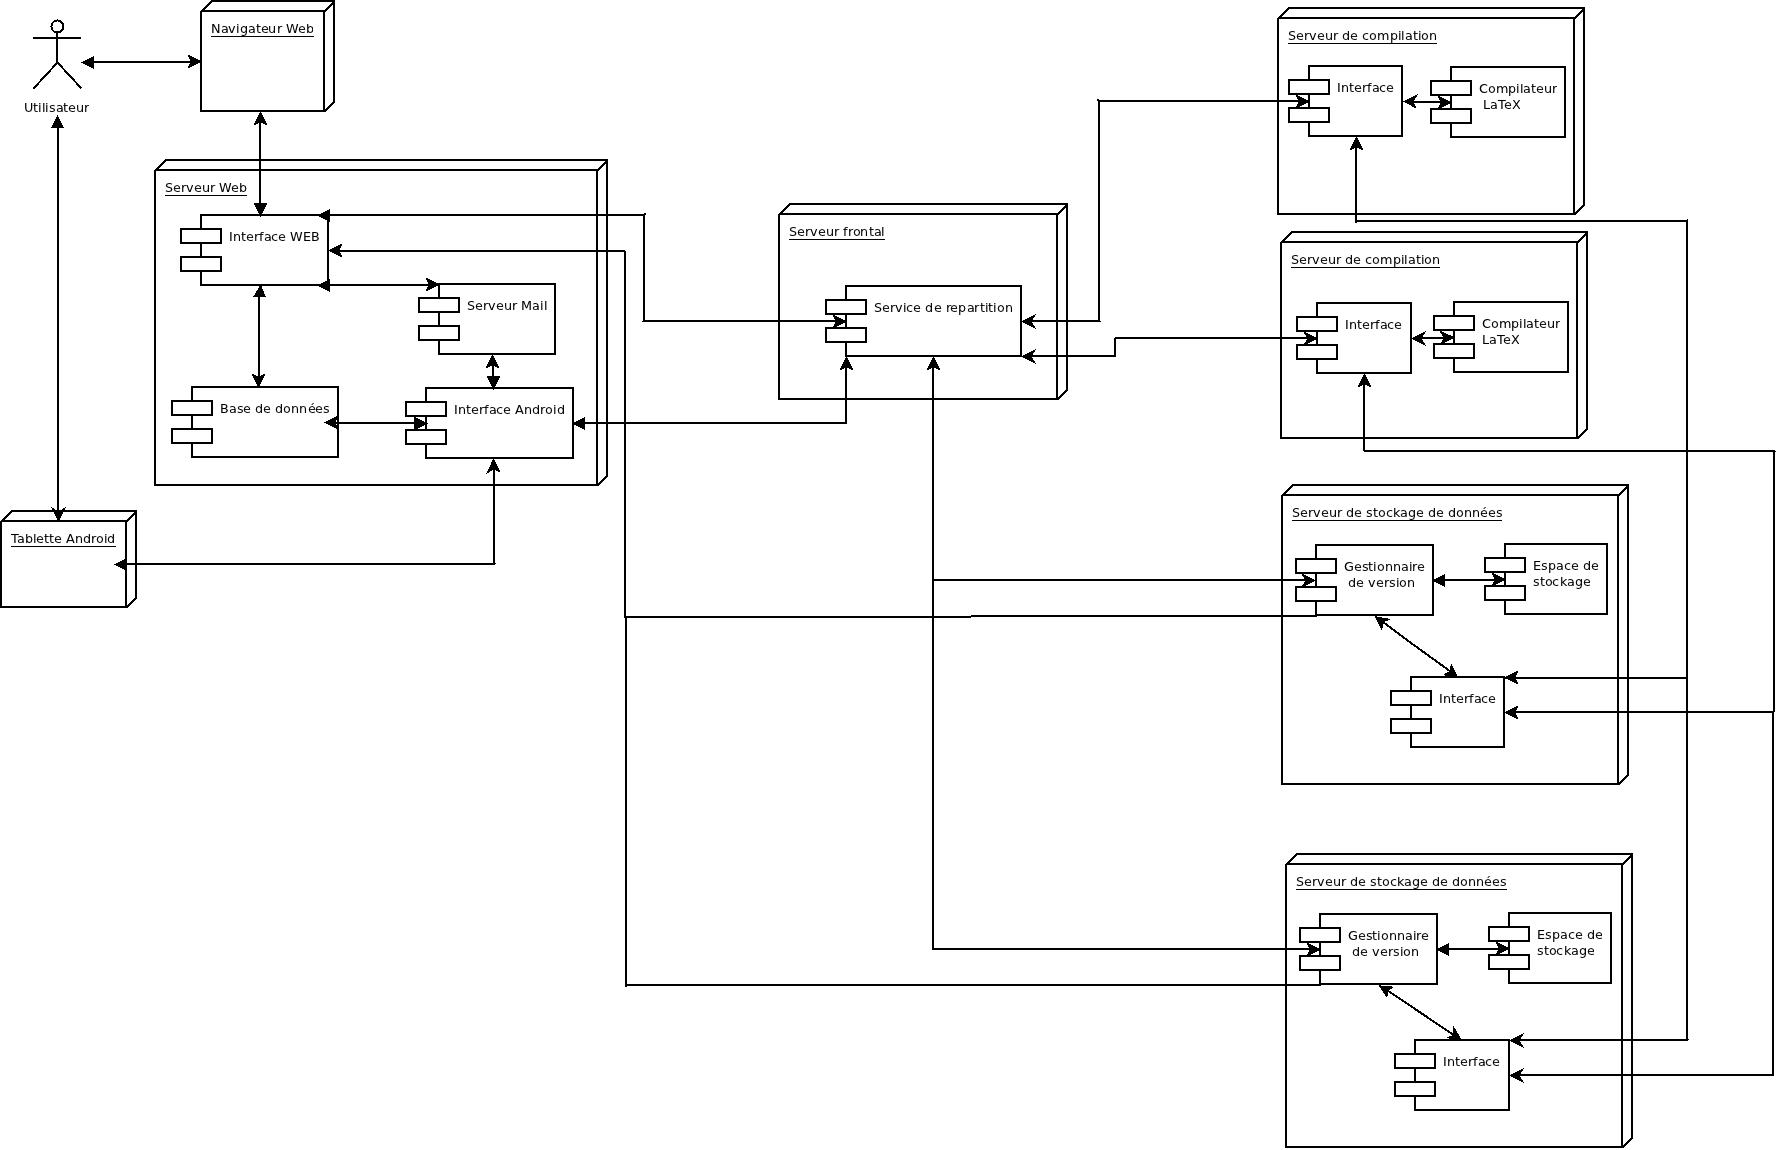
\includegraphics[width=0.92\textwidth,angle=90]{./images/DiagrammeDeploiement.jpg}
\end{center}
  \caption{Diagramme de déploiement}
  \label{déploiement}
\end{figure}

\paragraph*{}
Ce type d'architecture à été choisie car elle permet une extension du nombre de serveurs de compilation et de données théoriquement infinie. Aussi, elle permet de limité au maximum les échange "lourd"\footnote{Transfert de nombreux fichiers et donc potentiellement lourd pour le réseau}. L'ensemble des communications (sauf envoie de binaire) sont au format JSON.

\paragraph*{}
Typiquement une compilation de documents passe par l'ensemble des serveurs:
\begin{enumerate}
 \item Serveur HTTP $\rightarrow$ serveur de routage et d'ordonnancement
 \item Serveur routage et d'ordonnancement $\rightarrow$ serveur de stockage de données
 \item Serveur de stockage de données $\rightarrow$ serveur de compilation
 \item Serveur de compilation $\rightarrow$ serveur de stockage de données
 \item Serveur de stockage de données $\rightarrow$ serveur HTTP
\end{enumerate}



\subsection{Serveur web}
\paragraph*{}
Le serveur web inclue plusieurs services:
\begin{itemize}
 \item La base de données de l'application. Le SGBD MySQL a été choisie pour supporté cette tâche.
 \item L'interface coté serveur a été développé en PHP5. Le serveur HTTP Apache2 est utilisé pour géré les connexions.
 \item L'interface cliente utilise les technologies HTML5, CSS3 et javascript (Via le frameworks JQuery).
 \item L'interface de communication entre l'application Android et le reste de l'architecture.
\end{itemize}

\paragraph*{}
Un modèle de conception MVC a été utilisé afin de rendre le code de l'application plus clair, plus facilement maintenable et évolutif. Les communications avec le serveur de routage et d'ordonnancement sont effectués grâce à des sockets TCP qui ont une durée de vie égale à une boucle entre tous les serveurs. Ceci permet de ne pas laisser en permanence de ports ouvert sur le serveur et ainsi limité les risques d'attaques sur ce service.

\paragraph*{}
L'application Web est divisé en trois parties:
\begin{enumerate}
 \item La partie développement, où l'utilisateur peut écrire sont code LaTex, consulter les logs d'erreurs/warning (s'il existe) après la compilation.
 \item La partie gestion des projets. L'utilisateur peut crée des projets, des dossier (sous dossiers) et des fichiers LaTex. il peut aussi renommer, supprimer un projet, un dossier ou un fichier.
 \item La barre supérieur, où l'utilisateur peut synchronisées les fichiers qui ont été modifier, les compilées, télécharger sous format de PDF. Éventuellement l'utilisateur peut modifier ces informations personnels ou changer son mot de passe.
\end{enumerate}

\clearpage

\begin{figure}[!ht]
\begin{center}
  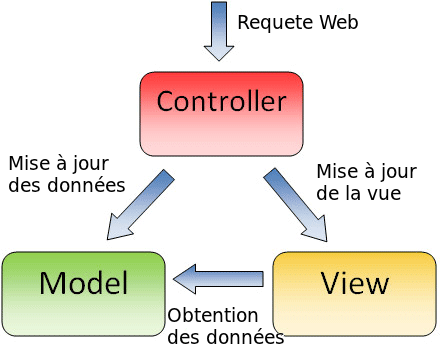
\includegraphics[width=0.6\textwidth]{./images/MVC.png}
\end{center}
  \caption{Diagramme MVC}
  \label{MVC}
\end{figure}

\subsection{Application Android}
\paragraph*{}
L'application Android comporte deux activités (écrans) principales.
\begin{itemize}
 \item La première est l'écran d'authentification, qui permet à l'utilisateur de s'authentifier afin d'accéder à son espace personnel, ou de s'inscrire afin de rejoindre le service TeXloud.
 \item La deuxième activité est lancée lorsque l'utilisateur est identifié. C'est l'écran principal de l'application.
\end{itemize}
\paragraph*{}

L'écran principal est divisé en trois parties : le bandeau supérieur, qui permet à l'utilisateur quelques interactions indispensables, comme la création de projet, la synchronisation ou encore la compilation. Lorsque l'utilisateur a fait des modifications qui 
n'ont pas été enregistrées (synchronisées), un logo rouge apparait pour rappeler à l'utilisateur de sauvegarder ses données. Une fois que les documents sont synchronisés, le logo rouge devient vert, l'utilisateur peut alors quitter l'application en étant sûr que ses 
modifications ont été prises en compte.
\paragraph*{}
La partie de gauche contient deux éléments : une liste déroulante (Spinner), qui permet à l'utilisateur de naviguer entre ses différents projets, et une arborescence qui permet à l'utilisateur de parcourir ses dossiers et fichiers. Un clic (appui) sur un dossier 
permet de masquer/afficher tous les fichiers et dossiers enfants (récursivement), et un clic sur un fichier le télécharge et l'affiche, permettant à l'utilisateur de le modifier. Les long clics sur les éléments de l'arborescence ouvrent un menu contextuel permettant, 
par exemple, d'ajouter un fichier, renommer, supprimer etc...
\paragraph*{}
La partie de droite est la saisie de texte. Le contenu de cette zone de texte est le contenu du fichier ouvert, affiché en italique dans l'arborescence de droite.Pour des raisons de simplicité, les ordres de synchronisation et de compilation sont bloquants, c'est-à-dire que l'utilisateur ne peut effectuer aucune modification tant que ces actions ne sont pas terminées.Toutes les requêtes utilisent le protocole HTTP et envoie les données via POST.


\subsection{Serveur de routage et d'ordonnancement}
\paragraph*{}
Le serveur de routage et d'ordonnancement permet de géré les communications entre le serveur web et les différents serveur de données et de compilation. Ce service à été développé en python. Il fourni deux services:
\begin{enumerate}
 \item Un service de routage
 \item Un service d'ordonnancement
\end{enumerate}

\paragraph*{}
Le service de routage permet de dirigé les requêtes vers les bon serveurs en fonctions de l'action voulu (compilation vers un serveurs de compilation,gestion des données vers le bon serveur de données). Le service d'ordonnancement permet de répartir la charge sur les différents serveurs en fonction de leurs charge propre. L'ordonnancement permet ainsi d'éviter d'avoir des serveurs totalement au repos et d'autres au maximum de leurs capacité.

\paragraph*{}
Ce service permet de gérer plusieurs connexion simultané. Il a été mit en charge avec plus de 1000 connexions simultané et aucun problème n'as été constaté.

\paragraph*{}
Les communications entre le serveur HTTP, les serveurs de compilation et les serveurs de données sont effectués la aussi grâce à des socket TCP.

\paragraph*{}
L'ensemble des données sur les serveurs (adresse IP, port du service, type de service, charge maximal) sont stocké au sein d'un fichier XML sur ce serveur.


\subsection{Serveur de stockage de données}
\paragraph*{}
Lorsqu'un projet est crée sur TeXloud, un serveur de stockage lui est attribué lors de la création du projet par l'ordonnanceur.
Il s'agit en fait d'un parc de serveurs physiques disposant d'un démon serveur destiné à recevoir de la frontale des requêtes standardisées permettant de faire les traitements demandés.

L'application serveur est développée en python et dispose d'une socket en écoute sur un port spécifique.
La séparation des composant de l'application permet de donner un certaine scalabilité de l'application, les méthodes d'accès aux données peuvent donc différer selon le serveur concerné.
De plus, le stockage des fichier se fait à l'aide de gestionnaires de versions afin de permettre le travail en équipe et une gestion de version éventuelle.

\paragraph{}
Le service d'accès aux données se compose principalement de eux parties:

\begin{itemize}
\item Un démon serveur recevant les requêtes
\item Un connecteur permettant de faire les actions (notamment le stockage)
\end{itemize}

\paragraph{}
Chacune de ces parties sont implémentées par héritage, les deux classes \emph{DataSocket} et \emph{GenericConnector} définissent les méthodes nécessaires pour le fonctionnement complet du système et font éventuellement les traitements non spécifiques au type de stockage.
L'application est donc potentiellement capable d'ajouter des connecteurs spécifique pour un type de stockage différent en développant les fonctions nécessitant un traitement adapté à celui-ci.

Les fonctions du connecteur subversion sont intégrés par l'utilisation de la librairie Python PySvn permettant de faire les opération proposé par le système de gestion de version telle que les \emph{commit}, les \emph{merge} et les \emph{updates}.

\paragraph{}
Le concept de \emph{copies de travail} est au centre du système de gestion des données.
Les systèmes de gestions de versions permettent de récupérer une version d'un projet depuis un serveur distant en créant un \emph{miroir} du projet dans un état spécifique (généralement le dernier).

Le répertoire ainsi crée correspond à une copie de travail, lorsque des modification sont faites sur le projet, elles sont ajoutées puis mise à jour sur le serveur, créant ainsi une nouvelle version du projet.

\paragraph{}
\`A chaque connexion d'un utilisateur, une requête est envoyé par le serveur web jusqu'au serveur de donnée visé qui initialise une nouvelle copie de travail sur le serveur, il s'agit du répertoire de travail associé à l'utilisateur.
Les modifications effectuées au cours de la session de l'utilisateur sont synchronisées sur ce répertoire par écrasement des fichiers puis sont transmises aux gestionnaire de version.

\subsection{Serveur de compilation}
\paragraph*{}
Le serveur de compilation, comme son nom l'indique permet de compiler le projet LaTeX afin de générer un fichier PDF. Le processus du service de compilation se déroule en 5 étapes:
\begin{enumerate}
 \item Réception d'une archive qui contient tous les fichiers latex du projet
 \item Décompression de l'archive
 \item Compilation du projet\footnote{La gestion du nombre de compilation (édition des liens, bibtex,etc.) nécessaire est effectués par le script Perl latexmk}
 \item Génération d'un fichier de log au format XML
 \item Renvoi au serveur de données du log et du fichier PDF
\end{enumerate}

\paragraph{}
Ce service est la aussi développé en Python et les communications sont basé sur des socket TCP. De même que pour le service de routage et d'ordonnancement, le service de compilation peut gérer plusieurs connexion en simultané.


\newpage
\section{Utilisation des applications}
\subsection{Application Web}
\subsubsection{Création de compte}
\paragraph*{}

\subsubsection{Création de projet}
\paragraph*{}

\subsubsection{Compilation}
\paragraph*{}
\begin{itemize}
 \item Lancement compilation
 \item log
 \item visu du pdf
 \item telechargement du pdf
\end{itemize}


\subsubsection{Fonctions annexes}
\paragraph*{}
\begin{itemize}
 \item Suppression de dossier/fichier
 \item Rename dossier/fichier
 \item Info supp sur user
\end{itemize}

\subsection{Application Android}
\subsubsection{Création de compte}
\paragraph*{}

\subsubsection{Création de projet}
\paragraph*{}

\subsubsection{Compilation}
\paragraph*{}
\begin{itemize}
 \item Lancement compilation
 \item log
 \item visu du pdf
 \item telechargement du pdf
\end{itemize}


\subsubsection{Fonctions annexes}
\paragraph*{}
\begin{itemize}
 \item Suppression de dossier/fichier
 \item Rename dossier/fichier
 \item Info supp sur user
\end{itemize}

\newpage
\section{Perspective d'évolution}
\subsection{Support des images}
\paragraph*{}
Le supports des images dans l'application permettrai d'ajouter des images au sein des PDF généré. L'ajout de cette fonctionnalité est très simple et rapide à mettre en \oe uvre mais malheureusement, nous n'avons pas eu le temps de la mettre en place. Pour intégrer ce support, une légère modification de la frontale, du service web et de l'application Android sont nécessaire.

\subsection{Gestion des groupes}
\paragraph*{}
La gestion des groupes dans l'application permettrai la modification simultané de document par plusieurs utilisateurs. Cette modification est possible à intégrer par la suite car la base de données et le stockage des informations ont été prévue a cette effet\footnote{Le stockage des données étant effectués sur des serveur SubVersion et la gestion des conflit étant implémenté, la gestion des groupe ne posera aucun problème}. Comme pour le support des images, les modifications de l'application pour supporté cette fonctionnalité sont minime. Il s'agit seulement de modifier légèrement l'application Web et l'application Android.

\subsection{Coloration syntaxique sur Android}
\paragraph*{}
La coloration syntaxique sur tablette Android n'as pas été implémenté car nous n'avons pas trouvez de solution qui ne soit pas trop lourde en ressource pour une tablette. Ceci est sûrement possible si nous déclenchions la coloration syntaxique moins fréquemment, comme par exemple a chaque fin de ligne et juste sur la ligne en cour. Malheureusement nous n'avons pas eu le temps de mettre en place cette idée.

\subsection{Intégration de PDFJS}
\paragraph*{}
La librairie PDFJS\footnote{PDFJS est un librairie permettant d'afficher un PDF dans un canvas HTML5 grâce à du JavaScript} étant pour l'instant en version de développement, il nous a été impossible de l'intégrer directement au sein d'une page de TeXloud. Nous avons cherché pendant plus de 10 Heures pour l'intégrer mais le code ne contient aucune documentation et évolue de jour en jour.Le support serai possible mais demande des modifications très lourde des script de PDFJS. De ce fait nous pensons que lorsque une release stable sera produit par l'équipe de Mozilla, il sera plus simple de l'intégrer au sein de notre design.

\subsection{Mot de passe oublié}
\paragraph*{}
La gestion des mots de passes oubliés n'est pas encore implémentée puisqu'elle dépend de la gestion des e-mails, et nous n'avons pas développé cette fonction. Cependant, le bouton et la boite de dialogue sont déjà implémentés sur l'interface Android. La gestion des e-mails n'as pas été possible car nous n'avions pas l'architecture physique nous permettant de faire fonctionné convenablement un serveur mail\footnote{Pour être dans de bonne condition, il aurai fallu que nous puissions avoir un accès vers internet afin de contacté les serveur SMTP ou POP de différents fournisseur d'adresse mail}.

\subsection{Utilisation d'autre support de stockage}
\paragraph*{}
Il serait possible d'utiliser plusieurs gestionnaire de version différents, des systèmes de fichiers,etc. pour stocker les données des utilisateurs. Pour l'instant seul SubVersion est géré, mais grâce a une interface générique, il est possible de développer rapidement des connecteurs pour n'importe quel gestionnaire de version. Grâce à cette interface, il suffit juste de développer une classe fille de cette interface sur un serveur de stockage de données et faire les appels spécifique au gestionnaire de version voulu.

\newpage

\section{Conclusion}
\paragraph*{}



\newpage
\listoffigures


\end{document}
